\subsection{Simulated Annealing}

Simulated annealing is a stochastic algorithm that attempts to find the global optimum of an objective function $f(x)$. The method is inspired by statistical physics, in particular the Boltzmann distribution that specifies the probability of being in a particular state $x$:
\begin{equation}
    p(x) \propto \exp\{-f(x)/T\}
\end{equation}
where $f(x)$ is the energy of the system and $T$ is the temperature. As the temperature approaches zero, the system spends more and more time in its minimum energy (most probable) state. As the temperature decreases, the largest peaks become larger and the smallest peaks dissappear. By cooling slowly enough, it is possible to track the largest peak and therefore find the global optimum.\\

Simulated annealing is closely related to the Metropolis-Hastings algorithm for generating samples from a probability distribution. At each step of the algorithm, we sample a new state according to a proposal distribution $x^{\prime} \sim q(\dot|x_k)$, such as a random walk proposal:
\begin{equation}
    x^{\prime} = x_k + \epsilon_k, ~~~ \mathrm{where}~ \epsilon_k \sim N(0,\Sigma)
\end{equation}
Having proposed a new state, we compute $\alpha$ as in Algorithm \ref{alg:sim_annealing}.
\begin{algorithm}
\caption{Simulated Annealing}
\label{alg:sim_annealing}
\begin{algorithmic}[1]
\STATE $\alpha = \exp\{(f(x)-f(x^{\prime}))/T\}$
\STATE $r = \min(1,\alpha)$
\STATE $u \sim \mathrm{Unif}(0,1)$
\STATE if $u < r$ 
\STATE ~~~ $x_{k+1} = x^{\prime}$
\STATE else
\STATE ~~~ $x_{k+1} = x_k$
\STATE end if  
\end{algorithmic}
\end{algorithm}
Thus, if a new state has lower energy (higher probability), we will definitely accept it but if it has higher energy (lower probability), we might still accept it depending on the temperature. Therefore, the algorithm allows downhill moves in probability space but less frequently as the temperature drops. In practice it is common to use an exponential cooling schedule: $T_k = T_0 C^{k}$, where $T_0 \sim 1$ is the initial temperature and $C \sim 0.8$ is the cooling rate. Cooling too quickly can result in getting stuck in local optima, while cooling too slowly wastes time. The optimum cooling schedule is difficult to determine.    

\begin{figure}[tbhp]
    \centering
    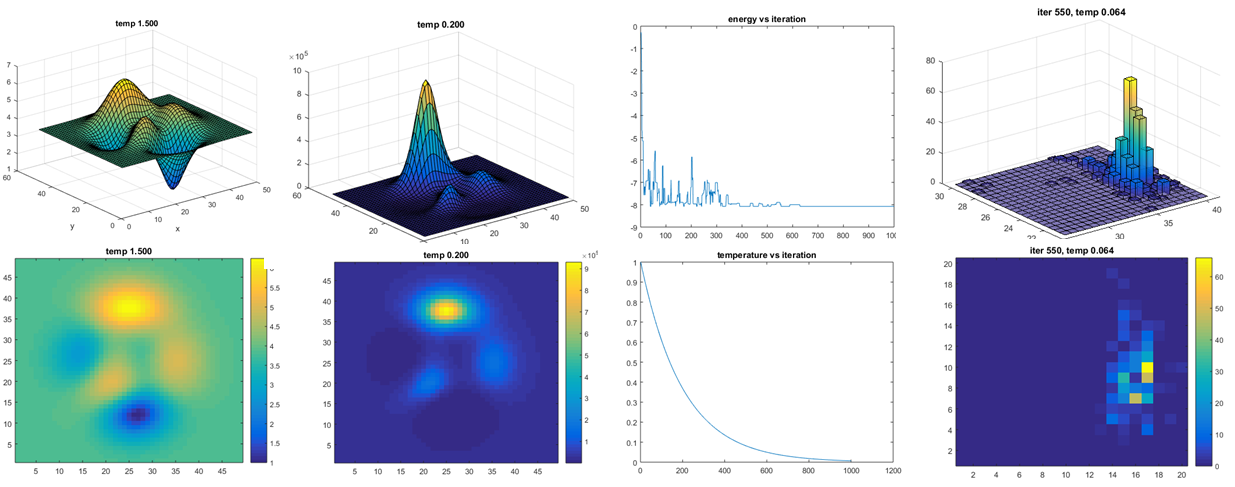
\includegraphics[width=0.9\textwidth, trim={10 10 10 10}]{figures/sim_annealing_merged.png}
    \caption{Simulated Annealing}
    \label{fig:sim_annealing_merged}
\end{figure}

Figure \ref{fig:sim_annealing_merged} shows the objective $f(x)$ at two different temperatures (left). The function appears more peaky when the temperature is lower. We can also see that the method stochastically reduces the energy over time for the given cooling schedule (middle). Finally a histogram of samples shows that most samples are concentrated near the global maximum (right).


\subsection{Bayesian Optimization}

Machine learning algorithms frequenty require careful tuning of hyperparameters. Often exhaustive and computationally expensive methods such as grid search cross validation are used to find model parameters that optimize a suitable performance objective. An alternative to grid search is randomized parameter optimization that samples parameter settings from a distribution over possible parameter values. This has two main benefits over the exhaustive search: the number of iterations can be chosen independent of the number of parameters and adding parameters that do not influence performance does not decrease efficiency. Rather than exploring the parameter space randomly (according to a chosen distribution), it would be great to adapt an active learning approach that selects parameter values in a way that reduces uncertainty and provides a balance between exploration and exploitation. Bayesian optimization provides an automated Bayesian framework by utilizing Gaussian Processes (GPs) to model algorithm's generalization performance \cite{snoek2012}.\\

Bayesian optimization assumes that a suitable performance function was sampled from a Gaussian Process and maintains a posterior distribution for this function as observations are made. To choose which hyperparameters to explore next, one can optimize the Expected Improvement (EI) over the current best result or the Gaussian process Upper Confidence Bound (UCB). EI and UCB have been shown to be efficient in the number of function evaluations required to find the global optimum of multi-modal black-box functions. Bayesian optimization uses all of the information available from previous evaluations of the objective function as opposed to relying on local gradient and Hessian approximations. This results in an automated procedure that can find an optimum of non-convex functions with relatively few evaluations, at the cost of performing more computation to determine the next point to try. This is particularly useful when evaluations are expensive to perform such as in selecting hyperparameters for deep neural networks.\\

To determine what point should be evaluated next, we need to choose and acquisition function which is used to construct a utility function from the GP posterior. In general, the acquisition function depends on previous observations as well as GP hyperparameters that we denote as $a(x;\{x_n,y_n\},\theta)$, then $x_{next} = \arg \max_x a(x)$. Let $\mu(x;\{x_n,y_n\},\theta)$ be the predictive GP mean function, $\sigma^{2}(x;\{x_n,y_n\},\theta)$ be the predictive GP variance function and $\Phi(x)$ be the cumulative distribution function of the standard normal. Then we can define the following acquisition functions.\\

\textit{Probability of Improvement}. This strategy maximizes the probability of improving over the best current value. This can be computed as follows:
\begin{equation}
    a_{PI}(x;\{x_n,y_n\},\theta) = \Phi(\gamma(x)), ~~~~ \gamma(x) = \frac{f(x_{best}) - \mu(x; \{x_n,y_n\},\theta)}{\sigma(x;\{x_n,y_n\},\theta)}
\end{equation}

\textit{Expected Improvement}. Alternatively, one could choose to maximize the expected improvement (EI) over the current best. 
\begin{equation}
    a_{EI}(x;\{x_n,y_n\},\theta) = \sigma(x;\{x_n,y_n\},\theta)(\gamma(x)\Phi(\gamma(x))+N(\gamma(x);0,1))
\end{equation}

\textit{Upper Confidence Bound}. UCB is the idea of exploiting upper confidence bounds to construct acquisition functions that minimize regret over the course of their optimization. These acquisition functions have the following form:
\begin{equation}
    a_{UCB}(x;\{x_n,y_n\},\theta) = \mu(x;\{x_n,y_n\},\theta) - \kappa \sigma(x;\{x_n,y_n\},\theta)
\end{equation}
where $\kappa$ is a tunable acquisition parameter to balance exploration and exploitation.\\


\begin{figure}[tbhp]
    \centering
    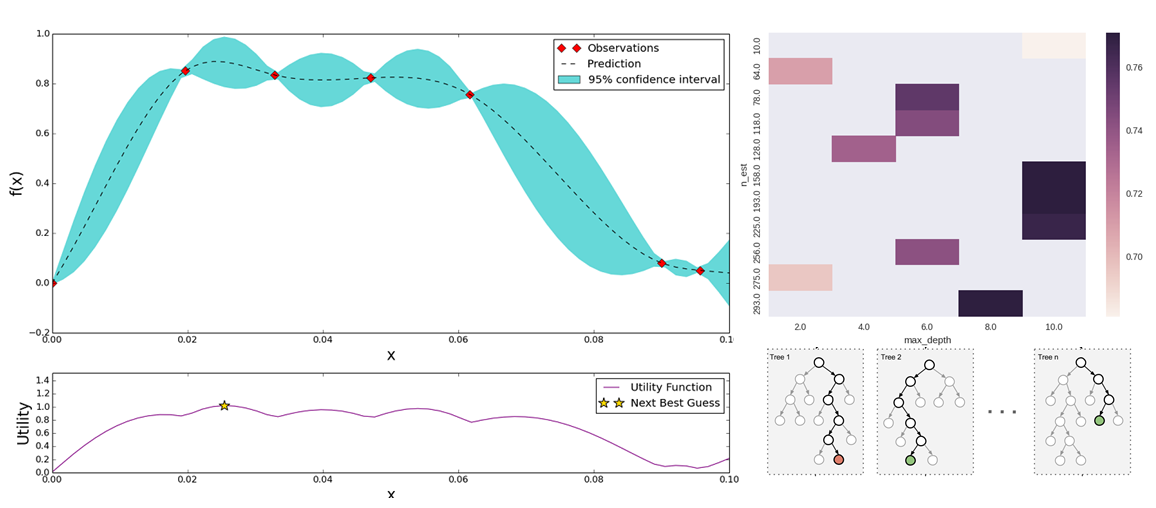
\includegraphics[width=0.95\textwidth, trim={10 10 10 10}]{figures/bayes_opt.png}
    \caption{Bayesian Optimization of SVM and Random Forest parameters}
    \label{fig:bayes_opt}
\end{figure}

Figure \ref{fig:bayes_opt} shows Baeysian optimization applied to SVM and Random Forest. F1 score was used as performance objective function for a classification task. The figure on the left shows Bayesian optimization of F1 score as a function of the gamma parameter of the SVM RBF kernel: $K(x,x^{\prime}) = \exp\{-\gamma ||x-x^{\prime}||^{2}\}$. We can see that after only 7 iterations we have discovered the gamma parameter that gives maximum F1 score. The peak of EI utility function at the bottom tells us which experiment to perform next. The figure on the right shows Bayesian optimization of F1 score as a function of maximum depth and the number of estimators of a Random Forest classifier. From the heatmap, we can tell that the maximum F1 score is achieved for $158$ estimators with depth equal to $10$.    
















